\newif\ifwide
\widetrue   % - 16:9 variant
%\widefalse  % - 4:3 variant
% For a 4:3 example, set aspectratio=43 and
% update all \includegraphics{} paths below for their 4:3 versions
% In the following examples, the correct variants are selected as
% \ifwide  (16:9 variant)  \else  (4:3 variant)  \fi

\ifwide
\documentclass[aspectratio=169]{beamer}
\else
\documentclass[aspectratio=43]{beamer}
\fi

\usetheme{tugraz2018}
\usepackage[english]{babel}


% two examples for logo-bars (few/many logos):
\newcommand{\myshortexamplelogobar}{Supported by:\qquad
    
\includegraphics[height=.5cm]{figures/logobarexample}\qquad
    
\includegraphics[height=.5cm]{figures/logobarexample}\qquad
    
\includegraphics[height=.5cm]{figures/logobarexample}%
}
\newcommand{\mylongexamplelogobar}{Supported by:\hfill\hfill
    
\includegraphics[height=.5cm]{figures/logobarexample}\hfill
    
\includegraphics[height=.5cm]{figures/logobarexample}\hfill
    
\includegraphics[height=.5cm]{figures/logobarexample}\hfill
    
\includegraphics[height=.5cm]{figures/logobarexample}\hfill
    
\includegraphics[height=.5cm]{figures/logobarexample}%
}


\begin{document}

%%%%%%%%%%%%%%%%%%%%%%%%%%%%%%%%%%%%%%%%%%%%%%%%%%%%%%%%%%%%%%%%%%%%%%%%%%%%%%%%

% TITLE
\begin{frame}[plain]
  \subtitle{Examples: Welcome}
  \title{Cover slide design for events (16:9 or 4:3)}
  \instituteurl{cd.tugraz.at}
  \makewelcome
\end{frame}

%%%%%%%%%%%%%%%%%%%%%%%%%%%%%%%%%%%%%%%%%%%%%%%%%%%%%%%%%%%%%%%%%%%%%%%%%%%%%%%%

% EXAMPLE 1: default (gray background with Alte Technik outline, text below the bar)
\begin{frame}[plain]
  \subtitle{Willkommen! / Welcome!}
  \title{Name der Veranstaltung und Zusatzinformationen / \\ Event Title and Information}
  \date{Datum / Date \\
        Ort / Location}
  \additionallogo{figures/logoinstituteexample} % optional

  \makewelcome
\end{frame}

%%%%%%%%%%%%%%%%%%%%%%%%%%%%%%%%%%%%%%%%%%%%%%%%%%%%%%%%%%%%%%%%%%%%%%%%%%%%%%%%

% EXAMPLE 2: with photo (Alte Technik) on top
\begin{frame}[plain]
  % select page style and data
  \ifwide % if 16:9:
    \titlefigure{figures/topfigureexample-169}
  \else % if 4:3:
    \titlefigure{figures/topfigureexample-43}
  \fi
  \setbeamercolor{tuglogo}{fg=white}  % TU Graz logo with white text

  % define page content
  \subtitle{Willkommen! / Welcome!}
  \title{Name der Veranstaltung und Zusatzinformationen / \\ Event Title and Information}
  \date{Datum / Date \\
        Ort / Location}

  % draw page
  \makewelcome

  % place additional logos, markers, etc.
  \begin{tikzpicture}[tugtheme]
    % event logo (bottom right):
    \draw (bottextSE) node[above left] {
\includegraphics[width=3.5cm]{figures/logoexample1}};
    % image copyright:
    \draw (topcopyrightSE) node[above left, copyright] {\copyright\ Lunghammer -- TU Graz};
  \end{tikzpicture}
\end{frame}

%%%%%%%%%%%%%%%%%%%%%%%%%%%%%%%%%%%%%%%%%%%%%%%%%%%%%%%%%%%%%%%%%%%%%%%%%%%%%%%%

% EXAMPLE 3: with photos (montage) on top
\begin{frame}[plain]
  \ifwide
    \titlefigure{figures/topfigureexample-montage-169}
  \else
    \titlefigure{figures/topfigureexample-montage-43}
  \fi
  \colorlet{main}{titleblue}

  \subtitle{Herzlich Willkommen!}
  \title{Name der Veranstaltung / \\ Event Title}
  \date{Datum / Date, Ort / Location}
  \logobar{\mylongexamplelogobar\hspace*{.7cm}\null}
  \instituteurl{www.tugraz.at/go/events}

  \makewelcome

  \begin{tikzpicture}[tugtheme]
    % event logo:
    \draw (bottextaltNE) node[below left] {
\includegraphics[width=3.5cm]{figures/logoexample1}};
    % image copyright:
    \draw (topcopyrightSE) node[above left, copyright] {\copyright\ Lunghammer -- TU Graz};
  \end{tikzpicture}
\end{frame}

%%%%%%%%%%%%%%%%%%%%%%%%%%%%%%%%%%%%%%%%%%%%%%%%%%%%%%%%%%%%%%%%%%%%%%%%%%%%%%%%

% EXAMPLE 4: with gradient gray background and logo on top
\begin{frame}[plain]
  \setbeamertemplate{welcome page top}[shade]

  \subtitle{Herzlich Willkommen!}
  \title{Name der Veranstaltung / \\ Event Title}
  \date{Datum / Date\\
        Ort / Location}

  \makewelcome

  \begin{tikzpicture}[tugtheme]
    % event logo:
    \draw (toptextSW) node[above right] {
\includegraphics[width=6.25cm]{figures/logoexample1}};
  \end{tikzpicture}
\end{frame}

%%%%%%%%%%%%%%%%%%%%%%%%%%%%%%%%%%%%%%%%%%%%%%%%%%%%%%%%%%%%%%%%%%%%%%%%%%%%%%%%

% EXAMPLE 5: with solid dark blue background and logo on top
\begin{frame}[plain]
  \setbeamertemplate{welcome page top}[fill]
  \setbeamercolor{tuglogo}{fg=white}

  \subtitle{Herzlich Willkommen!}
  \title{Name der Veranstaltung / \\ Event Title}
  \date{Datum / Date\\
        Ort / Location}

  \makewelcome

  \begin{tikzpicture}[tugtheme]
    % event logo:
    \draw (toptextSW) node[above right] {
\includegraphics[width=6.25cm]{figures/logoexample1}};
  \end{tikzpicture}
\end{frame}

%%%%%%%%%%%%%%%%%%%%%%%%%%%%%%%%%%%%%%%%%%%%%%%%%%%%%%%%%%%%%%%%%%%%%%%%%%%%%%%%

% EXAMPLE 6: with solid light background and logo on top
\begin{frame}[plain]
  \setbeamercolor{welcome page top}{fg=black,bg=titlelite} % set top background color to light color
  \setbeamertemplate{welcome page top}[fill]
  \colorlet{main}{titledark} % set welcome bar color

  \subtitle{Welcome!}
  \title{Name der Veranstaltung / \\ Event Title}
  \date{Datum / Date, Ort / Location}
  \logobar{\myshortexamplelogobar}

  \makewelcome

  \begin{tikzpicture}[tugtheme]
    \ifwide % 16:9 variant:
      % event logo:
      \draw (toptextSW) node[above right] {
\includegraphics[width=5.75cm]{figures/logoexample2}};
      % custom image and copyright information:
      \draw (toprightlogoSE) node[above left] {
\includegraphics[width=7.0cm]{figures/photoexample-169}}
            ++(-7,0)         node[above right, copyright] {\copyright\ Lunghammer -- TU Graz};
    \else % 4:3 variant:
      % event logo:
      \draw (toptextSW) node[above right] {
\includegraphics[width=4.75cm]{figures/logoexample2}};
      % custom image and copyright information:
      \draw (toprightlogoSE) node[above left] {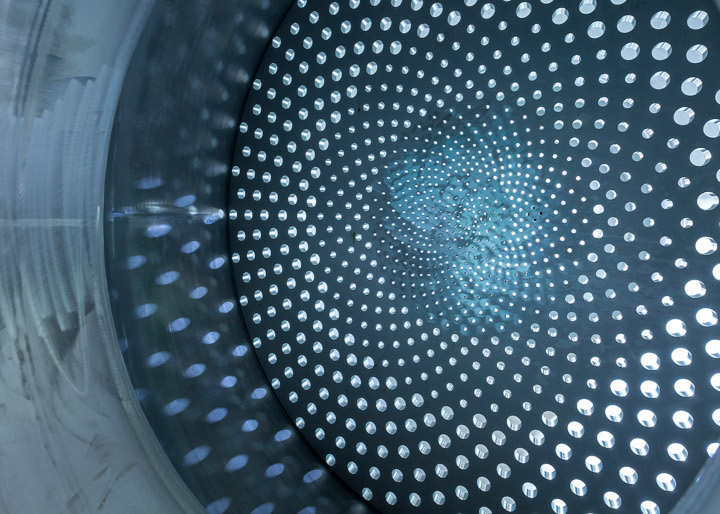
\includegraphics[width=6.0cm]{figures/photoexample-43}}
            ++(-6,0)         node[above right, copyright] {\copyright\ Lunghammer -- TU Graz};
    \fi
  \end{tikzpicture}
\end{frame}

%%%%%%%%%%%%%%%%%%%%%%%%%%%%%%%%%%%%%%%%%%%%%%%%%%%%%%%%%%%%%%%%%%%%%%%%%%%%%%%%

% AVAILABLE TikZ COORDINATES
\begin{frame}[plain]
  \subtitle{Available Coordinates}
  \date{Rectangle corners: \texttt{NW} (labelled, e.g., \texttt{topNW}), \texttt{SW}, \texttt{NE}, \texttt{SE}}

  \makewelcome

  \begin{tikzpicture}[tugtheme,font=\ttfamily\small,thick]
    \draw (topNW) node[below right] {top} rectangle (topSE);
    \draw (toptextNW) node[below right] {toptext/toptextalt} rectangle (toptextSE)
          (toptextNW) rectangle (toptextaltSE);
    \draw (barNW) node[below right] {bar} rectangle (barSE);
    \draw (bartextNW) node[below right] {bartext} rectangle (bartextSE);
    \draw (botNW) node[below right] {bot} rectangle (botSE);
    \draw (footNW) node[below right] {foot} rectangle (footSE);
    \draw (bottextNW) node[below right] {bottext/bottextalt} rectangle (bottextSE)
          (bottextNW) rectangle (bottextaltSE);
    \draw (toprightlogoSE) node[fill,circle,minimum size=3pt] {} node[above left] {toprightlogoSE};
    \draw (topcopyrightSE) node[fill,circle,minimum size=3pt] {} node[above left] {topcopyrightSE};
  \end{tikzpicture}
\end{frame}

\end{document}
